 % !TEX root = article.tex

\section{Experimental Evaluation}
\label{se:experiments}

In this section we present a preliminar experimental study of \osrkit\ aimed at addressing the following questions:
\ifdefined \noauthorea
\begin{description}
\else
\begin{description}
\fi
\item[Q1] How much does a never-firing OSR point impact code quality? What kind of slowdown should we expect?
\item[Q2] What is the run-time overhead of an OSR transition, for instance to a clone of the running function?
\item[Q3] What is the overhead of \osrkit\ for inserting OSR points and creating a stub or a continuation function?
\item[Q4] What kind of benefits can we expect by using OSR in a production environment based on LLVM?
\end{description}

\subsection{Benchmarks and Setup}
We address questions Q1-Q3 by analyzing the performance of \osrkit\ on a selection of the \shootout\ benchmarks~\cite{shootout} running in a proof-of-concept virtual machine we developed in LLVM. In particular, we focus on single-threaded benchmarks that do not rely on external libraries to perform their core computations. Benchmarks and their description are reported in \mytable\ref{tab:shootout}; four of them ({\tt b-trees}, {\tt mbrot}, {\tt n-body} and {\tt sp-norm}) are evaluated against two workloads of different size.

%In this section we present a preliminar experimental study of our OSR implementation in TinyVM. Our experiments are based on the \shootout\ test suite, also known as the Computer Language Benchmark Game~\cite{shootout}. In particular, we focus on single-threaded benchmarks that do not rely on external libraries to perform their core computations.

%, a proof-of-concept virtual machine based on LLVM's JIT compiler MCJIT. TinyVM supports interactive invocations of functions and it can compile LLVM IR either generated at run-time or loaded from disk. The main design goal behind TinyVM is the creation of an interactive environment for IR manipulation and JIT-compilation of functions: for instance, it allows the user to insert OSR points in loaded functions, run optimization passes on them or display their CFGs, repeatedly invoke a function for a specified amount of times and so on. TinyVM supports dynamic library loading and linking, and comes with a helper component for MCJIT that simplifies tasks such as handling multiple IR modules, symbol resolution in presence of multiple versions of a function, and tracking native code and other machine-level generated object such as Stackmaps.
%TinyVM is thus an ideal playground to exercise our OSR technique, and we use it to run performance measurements on the shootout test suite, also known as the Computer Language Benchmark Game~\cite{shootout}. 
%At the end of the section, we show experimental results for the case study presented in \mysection\ref{se:case-study}.

\begin{table}[hb]
\begin{center}
\begin{small}
\ifdefined \noauthorea
    \begin{adjustbox}{width=1\columnwidth}
\fi
    \begin{tabular}{ |c|c| }
        \hline
        Benchmark & Description \\ 
        \hline
        \hline
        b-trees & Adaptation of a GC bench for binary trees \\ 
        \hline
        fannkuch & Fannkuch benchmark on permutations \\ 
        \hline
        fasta & Generation of DNA sequences \\ 
        \hline
        fasta-redux & Generation of DNA sequences (with lookup table) \\ 
        \hline
        mbrot & Mandelbrot set generation \\ 
        \hline
        n-body & N-body simulation of Jovian planets \\ 
        \hline
        rev-comp & Reverse-complement of DNA sequences \\ 
        \hline
        sp-norm & Eigenvalue calculation with power method \\ 
        \hline
    \end{tabular} 
\ifdefined \noauthorea
    \end{adjustbox}
\fi
\end{small}
\end{center}
\caption{\label{tab:shootout} Description of the \shootout\ benchmarks.} 
\end{table}

%We generated the IR modules for our experiments with {\tt clang}, starting from the C version of the \shootout\ suite. In the version of the code we will refer to as {\em unoptimized}, no LLVM optimization passes were performed on the code other than {\em mem2reg}, which promotes memory references to register references and constructs the SSA (Static Single Assignment) form. Starting from this version, we then generate an {\em optimized} version performing using the LLVM IR optimizer {\tt opt} at {\tt -O1} optimization level.

\ifx\noauthorea\undefined
\medskip
\fi

\noindent We generate the IR modules for our experiments with {\tt clang} starting from the C version of the \shootout\ suite. To cover scenarios where OSR machinery is inserted in programs with different optimization levels, we consider two versions: 1) {\em unoptimized}, where the only LLVM optimization we perform is {\tt mem2reg} to promote stack references to registers and construct the SSA form; 2) {\em optimized}, where we apply {\tt opt} {\tt -O1} to the unoptimized version.

%In the version of the code we will refer to as {\em unoptimized}, the only LLVM optimization pass we perform is {\tt mem2reg}, which promotes stack references to registers and constructs the SSA form.
%\ifdefined \fullver
%Starting from this version, we also generate an {\em optimized} version using the LLVM IR optimizer {\tt opt} at {\tt -O1} optimization level.
%\else
%Starting from this version, we also generate an {\em optimized} version using the LLVM optimizer {\tt opt -O1}.
%\fi

For question Q4, we analyze the impact of the optimization technique presented in \mysection\ref{ss:eval-opt-mcvm} on the running time of a few numeric benchmarks, namely {\tt odeEuler}, {\tt odeMidpt}, {\tt odeRK4}, and {\tt sim\_anl}. The first three benchmarks~\cite{recktenwald2000numerical} solve an ordinary differential equation for heat treating simulation using the Euler, midpoint, and Range-Kutta method, respectively; the last benchmark minimizes the six-hump camelback function with the method of simulated annealing\footnote{\url{http://www.mathworks.com/matlabcentral/fileexchange/33109-simulated-annealing-optimization}}.

%\footnote{\url{http://web.cecs.pdx.edu/~gerry/nmm/mfiles/}}

All the experiments were performed on an octa-core 2.3 Ghz Intel Xeon E5-4610 v2 with 256+256KB of L1 cache, 2MB of L2 cache, 16MB of shared L3 cache and 128 GB of DDR3 main memory, running Debian Wheezy 7, Linux kernel 3.2.0,
\ifdefined \fullver
LLVM 3.6.2 (Release build, compiled using gcc 4.7.2), 64 bit.
\else
LLVM 3.6.2, 64 bit.
\fi

For each benchmark we analyze CPU time performing 10 trials preceded by an initial warm-up iteration; reported confidence intervals are stated at 95\% confidence level.


\subsection{Results}
\label{ss:experim-results}
%We now present the main results of our experimental evaluation, aimed at addressing the following questions:
%\begin{itemize}
%\item {\bf Message 1}: how much does a never-firing OSR point impact code quality? We run a program with one or more OSR points, and we measure the slowdown given by factors such as cache effects (due to code bloat), register pressure, etc. due to the presence of the OSR points.
%\item {\bf Message 2}: what is the overhead of an OSR transition to the same function? We run a program with a controlled OSR transition, e.g., with a counter that fires the OSR. Here we measure the impact of the actual OSR call. We compute for each benchmark: 1) the average time per OSR transition; 2) the number of transferred live variables; 3) the total benchmark time with an always-firing OSR at each iteration of the hottest loop; 4) the total benchmark time with a never-firing OSR at each iteration of the hottest loop (baseline); 5) the number of iterations of the hottest loop (equals the number of OSR transitions).
%\item {\bf Message 3}: what is the overhead of the library for inserting OSR points? We compute for each benchmark the time required by insertOpenOSR (OSR point insertion + stub creation) and insertFinalizedOSR (OSR point insertion + generation of continuation function).
%\end{itemize}

\begin{table*}[ht]
\begin{center}
\begin{small}
\ifdefined \noauthorea
    \begin{adjustbox}{width=1\textwidth}
\fi
    \begin{tabular}{ |c|c|c|c|c|c|c|c| }
        \cline{3-8}
        \multicolumn{2}{c|}{} & \multicolumn{3}{c|}{{\em Unoptimized version}} & \multicolumn{3}{c|}{{\em Optimized code}} \\
        \hline
        Benchmark & Fired OSR transitions & Live values & Avg time (ns) & Overhead (\%) & Live values & Avg time (ns) & Overhead (\%) \\ 
        \hline
        \hline
        b-trees & 605\,377\,887 & 2 & 1.731 & 3.96 & 3 & 0.974 & 2.29 \\ 
        \hline
        b-trees-large & 2\,689\,946\,975 & 2 & 1.749 & 3.90 & 3 & 1.423 & 3.30 \\ 
        \hline
        fannkuch & 399\,168\,000 & 0 & 1.793 & 1.73 & 0 & 0.621 & 0.59 \\ 
        \hline
        fasta & 400\,000\,000 & 2 & 2.335 & 7.39 & 2 & 2.699 & 8.23 \\ 
        \hline
        fasta-redux & 400\,000\,000 & 4 & 2.306 & 20.13 & 4 & 2.269 & 19.69 \\ 
        \hline
        mbrot & 256\,000\,000 & 15 & 5.016 & 2.40 & 15 & 3.628 & 1.75 \\ 
        \hline
        mbrot-large & 1\,024\,000\,000 & 15 & 5.268 & 2.53 & 15 & 4.637 & 2.25 \\ 
        \hline
        n-body & 50\,000\,000 & 3 & 2.952 & 1.65 & 3 & 6.929 & 3.59 \\ 
        \hline
        n-body-large & 500\,000\,000 & 3 & 2.953 & 1.64 & 3 & 6.953 & 3.60 \\ 
        \hline
        rev-comp & 6\,172\,843 & 8 & -10.158 & -1.10 & 8 & 8.267 & 0.92 \\ 
        \hline
        sp-norm & 1\,210\,000\,000 & 2 & 0.772 & 14.76 & 2 & -0.030 & -0.57 \\ 
        \hline 
        sp-norm-large & 19\,360\,000\,000 & 2 & 0.778 & 14.89 & 2 & -0.003 & -0.07 \\
        \hline
    \end{tabular} 
\ifdefined \noauthorea
    \end{adjustbox}
\fi
\end{small}
\end{center}
\caption{\label{tab:sameFun}Cost of OSR transitions to the same function. Overhead is assessed w.r.t. running time of the never-firing version. %For each benchmark we report the number of fired OSR transitions, the number of live values passed at the OSR point, the average time for performing a transition, and the slowdown of the always-firing w.r.t. the never-firing version calculated on total CPU time.
}
\end{table*}
\ifauthorea{\newline}{}


\paragraph{Q1: Impact on Code Quality.}
In order to measure how much a never-firing OSR point might impact code quality, we analyzed the source-code structure of each benchmark and profiled its run-time behavior to identify performance-critical sections for OSR point insertion. The distinction between open and resolved OSR points is nearly irrelevant in this context: we choose to focus on open OSR points, passing {\tt null} as the {\tt val} argument for the stub.

For iterative benchmarks, we insert an OSR point in the body of their hottest loops. We classify a loop as hottest when its body is executed for a very high cumulative number of iterations (e.g., from millions up to billions) and it either calls the method with the highest {\em self} time in the program, or it performs the most computational-intensive operations for the program in its own body.
\ifdefined \fullver
These loops are natural candidates for OSR point insertion: for instance, the Jikes RVM inserts yield points on backward branches to trigger operations such as method recompilation through OSR and thread preemption for garbage collection. In the \shootout\ benchmarks, the number of such loops is typically 1 (2 for {\tt spectral-norm}).
\else
These loops are natural candidates for OSR point insertion: for instance, the Jikes RVM inserts yield points on backward branches to trigger method recompilation through OSR or thread preemption for garbage collection. In the \shootout\ benchmarks, the number of such loops is typically 1 (2 for {\tt spectral-norm}).
\fi

For recursive benchmarks, we insert an OSR point in the body of the method that accounts for the largest {\em self} execution time in the program. Such an OSR point might be useful to trigger recompilation of the code at a higher degree of optimization, enabling for instance multiple levels of inlining for non-tail-recursive functions. The only analyzed benchmark showing a recursive pattern is {\tt b-trees}.

%For {\tt b-trees} - the only benchmark showing a recursive pattern - we insert an OSR point in the body of the method that accounts for the largest {\em self} execution time of the program. Such an OSR point might be useful to trigger recompilation of the code at a higher degree of optimization, or to enable some form of dynamic optimization (for instance, in a recursive search algorithm we might want to inline the comparator method provided by the user at the call).

Results for the unoptimized and optimized versions of the benchmarks are reported in \myfigure\ref{fig:code-quality-base} and \myfigure\ref{fig:code-quality-O1}, respectively. For both scenarios we observe that the overhead is very small, i.e. less than $1\%$ for most benchmarks and less than $2\%$ in the worst case. For some benchmarks, code might run slightly faster after OSR point insertion due to instruction cache effects.
%We analyzed the code produced by the x86-64 back-end: the OSR machinery is lowered into three native instructions that load a counter in a register, compare it against a constant value and jump to the OSR block accordingly.
The number of times the OSR condition is checked for each benchmark is 
%the same as in the experiments 
reported in \mytable\ref{tab:sameFun}.

% figure
\ifdefined\noauthorea
\begin{figure}[bh]
\begin{center}
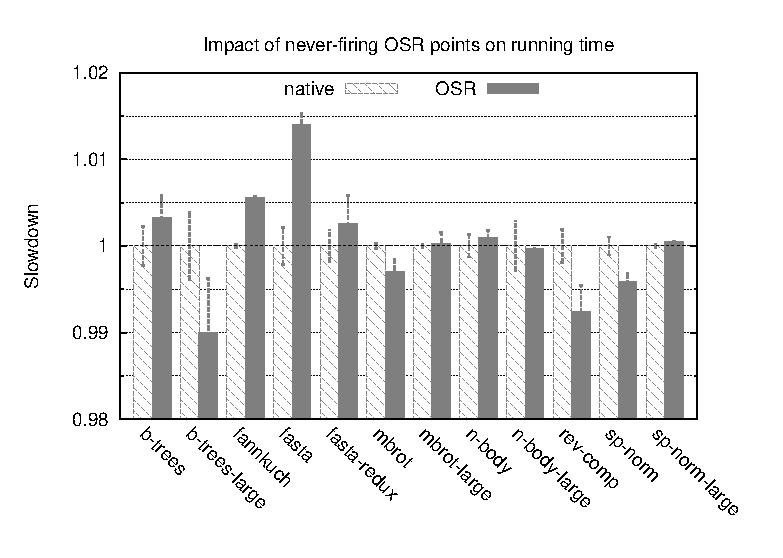
\includegraphics[width=0.95\columnwidth]{figures/code-quality-noBB/code-quality-noBB.eps}
\caption{\protect\label{fig:code-quality} Impact on running time of never-firing OSR points inserted inside hot code portions (unoptimized code).
  
  
  }
\end{center}
\end{figure}
\fi

% figure
\ifdefined\noauthorea
\begin{figure}[bh]
\begin{center}
%\vspace{-0.55cm}
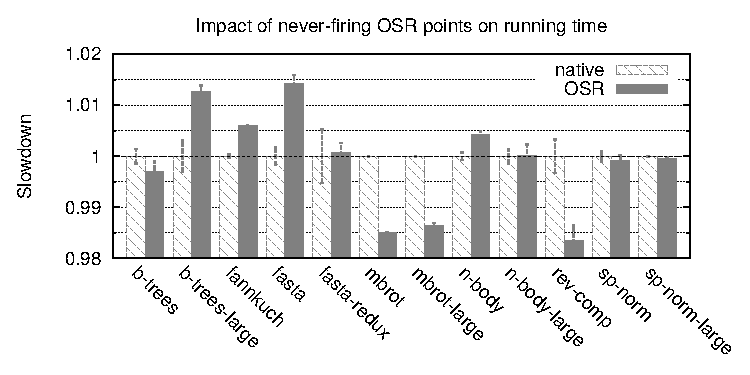
\includegraphics[width=0.95\columnwidth]{figures/code-quality-O1-noBB/code-quality-O1-noBB.eps}
\caption{\protect\label{fig:code-quality-O1} Impact on running time of never-firing OSR points inserted inside hot code portions (optimized code).
  
  
  
}
\end{center}
\end{figure}
\fi

\paragraph{Q2: Overhead of OSR Transitions.}

\mytable\ref{tab:sameFun} reports estimates of the average cost of performing an OSR transition to a clone of the running function. For each benchmark we compute the time difference between the scenarios in which an always-firing and a never-firing resolved OSR point is inserted in the code, respectively; we then normalize this difference against the number of fired OSR transitions.

Hot code portions for OSR point insertion have been identified as in Q1. %the experiments for code quality. 
\ifdefined\fullver %%%%%%
However, as for hot loops we want to perform an OSR transition at each iteration, inserting an always-firing OSR point in the enclosing function is not an option, because the function we OSR into should then fire an OSR itself, leading eventually to a very large number of active stack frames. 
\fi %%%%%%%%%%%%%
Depending on the characteristics of the hot loop, we either transform its body into a separate function and instrument its entrypoint, or, when the loop calls a method with a high self time, we insert an OSR point at the beginning of that method.

Normalized differences reported in the table represent a reasonable estimate of the average cost of firing an OSR transition.
%, which in other words is the cost of performing a function call passing the live variables as arguments. 
Reported numbers are in the order of nanoseconds, and might be negative due to instruction cache effects.

\paragraph{Q3: OSR Machinery Generation.}
We now discuss the overhead of the \osrkit\ library for inserting OSR machinery in the IR of a function. \mytable\ref{tab:instrTime} reports for each benchmark the number of IR instructions in the instrumented function and the time spent in the IR manipulation. Locations for OSR points are chosen as in 
%the experiments about code quality, 
Q1, and the target function is a clone of the source function.

For open OSR points, we report the time spent in inserting the OSR point in the function and in generating the stub; both operations do not depend on the size of the function. For resolved OSR points, we report the time spent in inserting the OSR point and in generating the \fosrto\ function.

Not surprisingly, constructing a continuation function takes longer than the other operations (i.e., up to 1 ms vs. 20-40 us), as it involves cloning and manipulating the body of the target function and thus depends on its size: \mytable\ref{tab:instrTime} thus comes with an additional column in which time is normalized against the number of IR instructions in the target.


\begin{table}[t]
\begin{small}
\ifdefined \noauthorea
    \begin{adjustbox}{width=1\columnwidth}
\fi
    \begin{tabular}{ |c|c|c|c|c|c|c| }
        \cline{3-7}
        \multicolumn{2}{l|}{} & \multicolumn{2}{c|}{{\em Open OSR {\tiny$(\mu s)$}}} & \multicolumn{3}{c|}{{\em Resolved OSR  {\tiny$(\mu s)$}}} \\ 
        \cline{3-7}
        \multicolumn{2}{l|}{} & Insert & Gen. & Insert & \multicolumn{2}{|c|}{Generate \fosrto} \\ 
        \cline{1-2} \cline{6-7}
        Benchmark & \textbar IR\textbar & point & stub & point & Total & Avg/inst \\
        \hline
        \hline
        b-trees & 13 & 15.40 & 28.32 & 14.31 & 76.13 & 5.86 \\
        \hline
        fannkuch & 50 & 14.16 & 18.66 & 12.84 & 208.03 & 4.16 \\
        \hline
        fasta & 38 & 12.93 & 27.07 & 13.01 & 250.39 & 6.59 \\
        \hline
        fasta-redux & 55 & 13.79 & 23.44 & 9.32 & 258.36 & 4.70 \\
        \hline
        mbrot & 77 & 15.96 & 27.39 & 15.30 & 384.61 & 4.99 \\
        \hline
        n-body & 19 & 14.31 & 19.73 & 11.58 & 88.73 & 4.67  \\
        \hline
        rev-comp & 145 & 16.31 & 39.99 & 13.90 & 810.84 & 5.59 \\
        \hline
        sp-norm & 28 & 15.31 & 27.50 & 12.41 & 154.54 & 5.52 \\ 
        \hline
    \end{tabular} 
\ifdefined \noauthorea
    \end{adjustbox}
\fi
\caption{\label{tab:instrTime} Q3: OSR machinery insertion in optimized code. Time measurements are expressed in microseconds. Results for unoptimized code are very similar and thus not reported.}
\end{small}
\end{table}
\ifauthorea{\newline}{}

\paragraph{Discussion.}
%Experimental results presented in this section suggest that inserting an OSR point is unlikely to degrade the quality of generated code, and the time required to fire an OSR transition is negligible (i.e., order of nanoseconds). Instrumenting the original IR is cheap, while the cost of generating a continuation function - either when inserting a resolved OSR point, or from the callback method invoked at an open OSR transition - is likely to be dominated by the cost of its compilation. For a front-end, the choice whether to insert an OSR point into a function for dynamic optimization depends on the trade-off between the expected benefits in terms of execution time and the overhead for generating on optimized version of the function and eventually JIT-compiling it; compared to these two operations, the cost of OSR-related operations is negligible.

Experimental results presented in this section suggest that inserting an OSR point is unlikely to degrade the quality of generated code (Q1). The time required to fire an OSR transition is negligible (i.e., order of nanoseconds, Q2), while the cost of OSR-point insertion and of generating a continuation function 
%- either when inserting a resolved OSR point, or from the callback method invoked at an open OSR transition - 
is likely to be dominated by the cost of its compilation (Q3). For a front-end, the choice whether to insert an OSR point into a function for dynamic optimization merely depends on the trade-off between the expected benefits in terms of execution time and the overheads from generating and JIT-compiling an optimized version of the function; compared to these two operations, the cost of OSR-related operations is negligible.

\begin{table}[h!]
\begin{small}
\ifdefined \noauthorea
    \begin{adjustbox}{width=1\columnwidth}
\fi
    % dirty hack for text wrapping
    \begin{tabular}{ |c|c|c|c|c| }
        \cline{2-5}
        \multicolumn{1}{c|}{} & Base & Optimized & Optimized & Direct \\ 
        \cline{1-1}
        Benchmark & (cached) & (JIT) & (cached) & (by hand) \\
        \hline
        \hline
        odeEuler & 1.046 & 2.796 & 2.800 & 2.828 \\ 
        \hline
        odeMidpt & 1.014 & 2.645 & 2.660 & 2.685 \\ 
        \hline
        odeRK4 & 1.005 & 2.490 & 2.582 & 2.647 \\ 
        \hline
        sim\_anl & 1.009 & 1.564 & 1.606 & 1.612 \\ 
        \hline
    \end{tabular} 
\ifdefined \noauthorea
    \end{adjustbox}
\fi
    \caption{\label{tab:feval} Q4: Speedup comparison for \feval\ optimization.} 
\end{small}
\end{table}

\paragraph{Q4: Optimizing {\tt feval} in MATLAB.}
%\label{sse:feval-results}
%We conclude this section with a discussion on the effectiveness of our optimization technique for McVM. In particular, we analyze its impact on the running time of a few numeric benchmarks, namely {\tt odeEuler}, {\tt odeMidpt}, {\tt odeRK4}, and {\tt sim\_anl}. The first three benchmarks solve an ODE for heat treating simulation using the Euler, midpoint, and Range-Kutta method, respectively\footnote{\url{http://web.cecs.pdx.edu/~gerry/nmm/mfiles/}}; the last benchmark minimizes the six-hump camelback function with the method of simulated annealing\footnote{\url{http://www.mathworks.com/matlabcentral/fileexchange/33109-simulated-annealing-optimization}}.
We report the speed-ups enabled by our technique in \mytable\ref{tab:feval}, using the running times for McVM's \feval\ default dispatcher as baseline. As the dispatcher typically JIT-compiles the invoked function, we also analyzed running times when the dispatcher calls a previously compiled function. In the last column, we show speed-ups from a modified version of the benchmarks in which each \feval\ call is replaced by hand with a direct call to the function in use for the specific benchmark.

Unfortunately, we are unable to compute direct performance metrics for the solution by Lameed and Hendren since its source code has not been released. Figures in their paper~\cite{lameed2013feval} show that for the very same MATLAB programs the speed-up of the OSR-based approach is on average within $30.1\%$ of the speed-up of hand-coded optimization (ranging from $9.2\%$ to $73.9\%$); for the JIT-based approach, the average grows to $84.7\%$ (ranging from $75.7\%$ to $96.5\%$).

Our optimization technique yields speed-ups that are very close to the upper bound given from by-hand optimization; in the {\em worst case} ({\tt odeRK4} benchmark), we observe a $94.1\%$ when the optimized code is generated on the fly, which becomes $97.5\%$ when a cached version is available. Compared to their OSR-based approach, the compensation entry block is a key driver of improved performance, as the benefits from a better type-specialized whole function body outweigh those from performing a direct call using boxed arguments and return values in place of the original \feval.



